\subsubsection{NATaS}
Pour paralléliser le SpMV, nous utilisons du parallélisme de boucle.
%
Notre ordonnanceur NUMA, NATaS, prend en charge ce type de parallélisme.
%
En plus d'optimiser le placement des pages, il répartira la charge de travail en prenant en compte la localité mémoire.
%
Sur le cas à 8 variables primaires, nous obtenons les mêmes performances qu'en mémoire distribuée (Fig.~\ref{fig:res_spmv_nas}).
%
Pour 3 variables primaires, nous obtenons 95~\% des performances de la version en mémoire distribuée.
%
Par contre, nous n'obtenons que 70~\% avec 1 variable primaire.

%   (-_-)   %
\begin{figure}[t!]
  \centering
  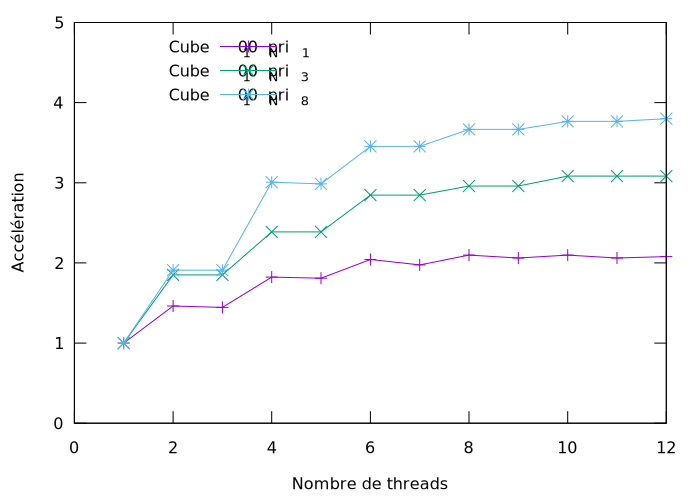
\includegraphics[width=0.7\textwidth]{res_spmv_nas}
  \caption{Accélération du produit matrice vecteur creux sur Rostand en mémoire partagée avec NATaS.}
  \label{fig:res_spmv_nas}
\end{figure}



Sur plusieurs bancs NUMA, NATaS offre des meilleures performances que l'ordonnanceur OpenMP même avec l'allocation mémoire interleaved.
%
{\em Croiser les doigts pour que ca fonctionne et donner résultat manumanu}
%
